%% ****** Start of file aiptemplate.tex ****** %
%%
%%   This file is part of the files in the distribution of AIP substyles for REVTeX4.
%%   Version 4.1 of 9 October 2009.
%%
%
% This is a template for producing documents for use with 
% the REVTEX 4.1 document class and the AIP substyles.
% 
% Copy this file to another name and then work on that file.
% That way, you always have this original template file to use.

%\documentclass[aip,graphicx]{revtex4-1}
%\documentclass[aip,reprint]{revtex4-1}

%\usepackage{graphicx}

%\draft % marks overfull lines with a black rule on the right
%\documentclass[pre,aps,floatfix,authordate1-4,twocolumn]{revtex4-1}
%\documentclass[pre,aps,floatfix,authordate1-4]{revtex4-1}

\documentclass[aps,prl,superscriptaddress,twocolumn]{revtex4}



%\documentclass[aps,prl,preprint,groupedaddress]{revtex4}

\usepackage{rotating} 
\usepackage{times}
\usepackage{graphicx}
\usepackage{setspace}
\usepackage{amsmath}
\usepackage{epstopdf}
\usepackage[obeyFinal]{easy-todo}
\usepackage{csquotes}
\usepackage{xr}
\externaldocument{manuscriptPSsuppl}

\begin{document}

% Use the \preprint command to place your local institutional report number 
% on the title page in preprint mode.
% Multiple \preprint commands are allowed.
%\preprint{}

\title{NMRlipids IV: Headgroup \& glycerol backbone structures, and cation binding in bilayers with PS lipids} %Title of paper

% repeat the \author .. \affiliation  etc. as needed
% \email, \thanks, \homepage, \altaffiliation all apply to the current author.
% Explanatory text should go in the []'s, 
% actual e-mail address or url should go in the {}'s for \email and \homepage.
% Please use the appropriate macro for the type of information

% \affiliation command applies to all authors since the last \affiliation command. 
% The \affiliation command should follow the other information.

\author{Tiago M. Ferreira}
\affiliation{Halle, Germany}
\author{Ivan Gushchin}
\affiliation{Moscow Institute of Physics and Technology}
\author{Matti Javanainen}
\affiliation{Institute of Organic Chemistry and Biochemistry,
Academy of Sciences of the Czech Republic, 
Prague 6, Czech Republic}
\author{Batuhan Kav}
\affiliation{Potsdam, Germany}
\author{Jesper J. Madsen}
\affiliation{Department of Chemistry, The University of Chicago, Chicago, Illinois 60637, United States of America}
\author{Markus Miettinen}
\affiliation{Potsdam, Germany}
\author{Josef Melcr}
\affiliation{Institute of Organic Chemistry and Biochemistry,
Academy of Sciences of the Czech Republic, 
Prague 6, Czech Republic}
\author{O. H. Samuli Ollila}
\email[]{samuli.ollila@helsinki.fi}
%\homepage[]{Your web page}
\affiliation{Institute of Organic Chemistry and Biochemistry,
Academy of Sciences of the Czech Republic, 
Prague 6, Czech Republic}
\affiliation{Institute of Biotechnology, University of Helsinki}
\author{Thomas Piggot   \todo{Authorlist is not yet complete}}
\affiliation{Southampton, United Kingdom}
%\author{NMRlipids collaboration}
%\affiliation{nmrlipids.blogspot.fi} 


% Collaboration name, if desired (requires use of superscriptaddress option in \documentclass). 
% \noaffiliation is required (may also be used with the \author command).
%\collaboration{}
%\noaffiliation

\date{\today}

\begin{abstract}
  % insert abstract here
Phosphatidylserine (PS) is the most common negatively
charged lipid in eykaryotic membranes.
PS lipids interact with signaling and other proteins via
electrostatic interactions and direct binding, and induce
membrane fusion and phase separation together with calcium ions.
Molecular details of these phenomena are not well understood
because accurate models to interpret the experimental data has not
been available. Here, we collect a set of experimental NMR data which
could be used together with molecular dynamics (MD) simulations
to interpret the lipid headgroup structures and details of ion binding
in pure and mixed PS and PS:PC lipid bilayers. Aiming to interpret the
data, we use the open collaboration method to go through the available MD simulation models for PS lipids.
However, none of the models reproduce the experimental data with sufficient
accuracy to interpet the structural details of lipid headgroups or
ion binding details in lipid bilayers containing PS lipids.
In contrast to PC lipids, the tested MD simulation models do not
correctly reproduce the qualitative response of PS lipid headgroups
to the bound ions or changes in the lipid composition. 
Our results pave the way for the model improvement to correctly
describe negatively charged membranes and their interactions with ions.
\end{abstract}

%\pacs{}% insert suggested PACS numbers in braces on next line

\maketitle %\maketitle must follow title, authors, abstract and \pacs

% Body of paper goes here. Use proper sectioning commands. 
% References should be done using the \cite, \ref, and \label commands


%\label{}
\section{Introduction}
Phosphatidylserine (PS) is the most common negatively
charged lipid in eykaryotic membranes.
PS lipids compose 8.5\% of total lipid weight of erythrocytes,
but the abundance varies between different organelles up to
25-35\% in plasma membrane \cite{lemmon08,leventis10,li14}.
Despite of the relatively low abundance, PS lipids
are important signaling molecules. They interact with
signaling proteins \cite{leventis10}, regulate
surface charge and protein localization \cite{yeung08}, and
induce protein aggregation \cite{zhao04,gorbenko06}.
Some domains spesifically interact PS lipids,
while others are attracted by general electrostatics and the
binding can be regulated by calcium \cite{leventis10}.
Therefore, the structural details
of lipid headgroups and the details of cation binding
are crucial for the PS mediated signaling processes.

Previous experimental studies have concluded that
PS headgroups are more rigid than phophocholines (PC)
due to the hydrogen bonding network or
electrostatic interactions \cite{browning80,buldt81}.
Multivalent cations and Li$^+$ are able to form strong
dehydrated molecular complexes with PS lipids,
while monovalent ions interact more weakly with PS
containing bilayers \cite{hauser77,kurland79,eisenberg79,hauser83,dluhy83,hauser85,feigenson86,mattai89,roux90,roux91,boettcher11}.
The dehydrated complexes of PS headgroup and calcium ions can also lead to the
phase separation \cite{hauser77,kurland79,hauser85,feigenson86,mattai89,roux90,roux91}.
On the other hand, some studies propose that the specific binding
affinity is similar to the negatively charged and zwitterionic lipids and that
the increased cation binding to negatively charged lipid bilayer arise only due
to the increase of local cation concentration in the vicinity of membranes \cite{seelig90,sinn06}.
Dilution of bilayers with PC lipids makes PS headgroups
less rigid and reduces propensity for the formation of
strong complexes with multivalent ions \cite{browning80,buldt81,roux90,roux91}.
The molecular level interpretation of these observations is,
however, not available.

Several classical molecular dynamics (MD) simulation studies are done
to understand PS headgroups, their influence on lipid bilayer properties and
interactions with ions \cite{cascales96,pandit02,mukhopadhyay04,pedersen06,vernier09,boettcher11,molina12,jurkiewicz12,venable13,pan14,vangaveti14,melcrova16}.
However, the recent comparisons of PC lipid headgroup and glycerol backbone
C-H bond order parameters calculated from different simulation models
revealed that improvements in the current force fields are needed
to correctly reproduce the headgroup structure and ion binding to
lipid bilayers \cite{botan15,catte16,ollila16}. The ion binding affinity
to POPC bilayer was then improved by implicitly including the electronic
polarizability using the electronic continuum correction \cite{melcr18}.
Here, we collect the set of experimentally measured lipid headgroup and
glycerol backbone C-H bond order parameters, which can be used to
evaluate the quality of headgroup structure and the ion binding affinity
in MD simulations of lipid bilayers containing PS lipids. 
The available MD simulation models of PS are then compared against
the collected experimental data. The results pave the way for the
development of MD simulation force fields that correctly describe
PS lipid headgroup structure and its interactions with ions.
Such models are expected to be useful in elucidating the biological
role of PS and other lipid headgroups because glycerol backbone and
lipid headgroups behave similarly in model membranes and in
bacteria \cite{gally81,scherer87,seelig90}.


%In NMRlipids I and II project we were looking for a MD model
%which would correctly reproduce headgroup and glycerol
%backbone structures and cation binding for PC lipid bilayers \cite{botan15,catte16}.
%Here we extend the same goal for lipids with negatively charged PS headgroup.
%Chemical structure of PS headgroup together with other common biological
%lipids is shown in Fig. \ref{lipids}.
%\begin{figure}[]




%  \centering
%  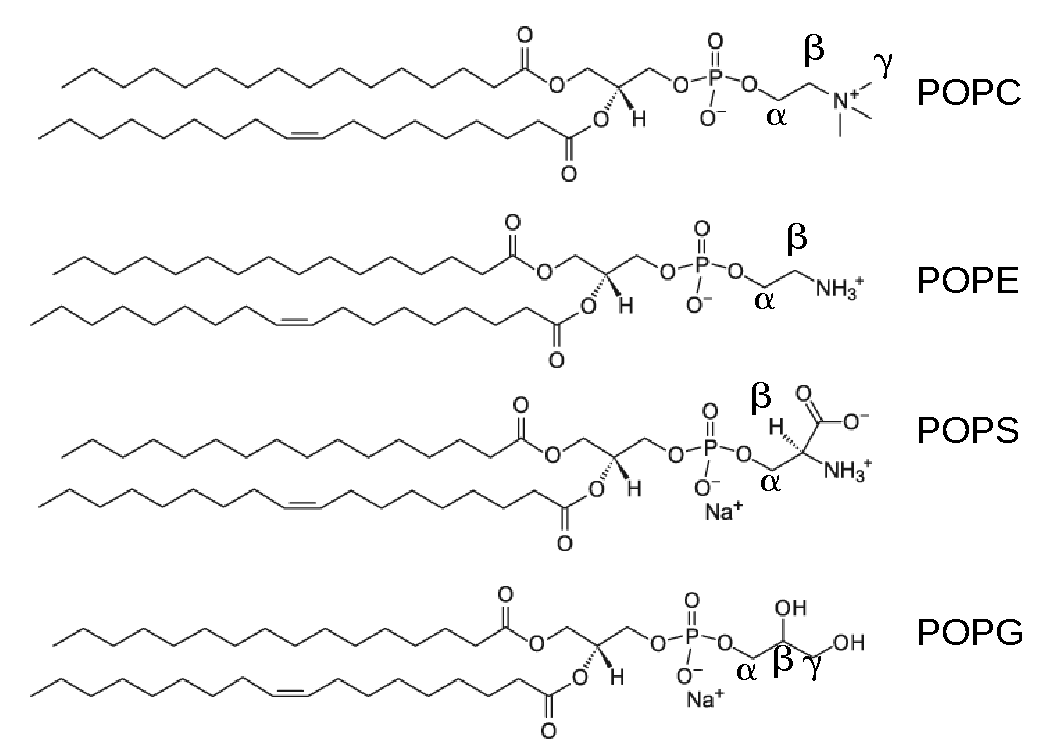
\includegraphics[width=9.0cm]{../Figs/lipids.pdf}
%  \caption{\label{lipids}
%    Chemical structures and labels for the headgroup carbons.
%  }
%\end{figure}


%The interpretation of this data and some other results has been that \cite{seelig90}
%\begin{displayquote}
%  {\it ''(i) Ca$^{2+}$ binds to neutral lipids (phosphatidylcholine, phosphatidylethanolamine) and negatively charged lipids
%    (phosphatidylglycerol) with approximately the same binding constant of K = 10-20 M$^{-1}$; \\
%    (ii) the free Ca$^{2+}$
%    concentration at the membrane interface is distinctly enhanced if the membrane carries a negative surface
%    charge, either due to protein or to lipid; \\
%    (iii) increased inter-facial Ca$^{2+}$ also means increased amounts
%    of bound Ca$^{2+}$ at neutral and charged lipids; \\
%    (iv) the actual binding step can be described by a Langmuir
%    adsorption isotherm with a 1 lipid:1 Ca$^{2+}$ stoichiometry, provided the interfacial concentration C$_M$, is
%    used to describe the chemical binding equilibrium.''}
%\end{displayquote}




%Phospholipids containing various polar headgroups and acyl
%chains are essential building blocks of biological membranes.
%Atomistic level structural details of lipids and lipid-ion 
%interactions are considered highly important in several
%biological processes. The lipid structure and ion binding
%can be studied in detail with NMR spectroscopy. However,
%the structural interpretation of NMR data requires usage
%of models. The combination of classical molecular dynamics
%simulations with NMR data, especially with C-H bond
%order parameters, can potentially give atomistic resolution
%interpretation of structure and dynamics of molecules \cite{botan15,ollila16,ferreira16}. 

%Our recent studies concluded that MD models are cabable to
%give structural interpretation for phosphatidylcholine 
%hydrophopic acyl chain region, while hydrophilic headgrop, glycerol 
%backbone and cation binding posed a major challenge for current
%force fields \cite{botan15,ollila16,catte16,ferreira16}. 
%These conclusions were reached by reviewing extensively 
%available experimental data from various sources and using
%NMRlipids Open Collaboration project to collect massive 
%amount of simulation data \cite{botan15,catte16}.

%Here we apply the same approach in search of MD simulation
%models which would reproduce glycerol backbone and 
%headgroup structures of lipids with PE, PG and PS headgroups.  
%In addition, we attempt to find a MD simulation model
%that would be able to correctly describe cation binding in
%bilayer containing negatively charged PG and PS lipids.


%Several MD simulation models have succesfully described 
%acyl chain structures and their qaulitative changes in different
%conditions for phosphatidylcholine lipids (for review see \cite{ollila16}).
%However, the current simulation models were not found to be accurate
%enough for full structural interpretation of phosphatidylcholine headgroup and
%glycerol backbone \cite{botan15}. Also Na$ +$  binding affinities
%were found to be significantly overestimated in several models and 
%none of the available models was able to Ca$2+$ 


\begin{table*}[!htb]
%\begin{sidewaystable*}[!p]
\centering
\caption{List of MD simulations of pure PS bilayers without additional salt.
   CKPM refers to the version with Berger/Chiu NH$_3$ charges compatible with Berger
   (i.e. the NH$_3$ group having the same charges as in the N(CH$_3$)$_3$ group of the PC lipids;
   'M' stands for Mukhopadhyay after the first published Berger-based PS simulation that used these charges~\cite{mukhopadhyay04})
   and CKP refers to the version with more Gromos compatible version
   (i.e. the charges for the NH$_3$ group taken from the lysine side-chain).
   %   these correspond the concentrations reported in the experiments by Akutsu et al.~\cite{akutsu81}.
   %   The lipid force fields named as in our previous work~\cite{botan15}.
}\label{PSsystems}
%begin{minipage}[t]{\textwidth}
\begin{tabular}{l c r r r r r c c}
  %\hline
  % some footnotes are not visible in typeset-MS (pdf)
 lipid/counter-ions & force field for lipids / ions & \footnote{Number of lipid molecules with largest mole fraction}N$_{\rm l}$   &  \footnote{Number of water molecules}N$_{\rm w}$  & \footnote{Number of additional cations}N$_{\rm c}$  & \footnote{Simulation temperature}T (K)  & \footnote{Total simulation time}t$_{{\rm sim}}$(ns) & \footnote{Time used for analysis}t$_{{\rm anal}}$ (ns) &   \footnote{Reference for simulation files}files\\
  \hline
    DOPS/Na$^+$  & CHARMM36 \cite{venable13}       & 128 & 4480 & 0  & 303  & 500 & 100 & \cite{charmm36DOPS303K} \\
    DOPS/Na$^+$  & CHARMM36ua \cite{??} \todoi{Correct citation for CHARMMua DOPS}   & 128 & 4480 & 0  & 303  & 500 & 100 & \cite{charmm36uaDOPS303K} \\
    DOPS/Na$^+$  & Slipids \cite{jambeck13}        & 128 	& 4480  & 0  & 303  & 500 & 100 & \cite{slipidsDOPS303K} \\
    DOPS/Na$^+$  & Slipids \cite{jambeck13}        & 288 	& 11232 & 0  & 303  & 200 & 100 & \cite{slipidsDOPSfiles} \\
    DOPS/Na$^+$  & Berger \cite{mukhopadhyay04}    & 128  & 4480  & 0  & 303  & 500 & 100 & \cite{bergerDOPS303K} \\
    DOPS/Na$^+$  & GROMOS-CKP1 \cite{??} \todoi{Correct citation(s) for CKP.} & 128 & 4480 & 0  & 303  & 500 & 100 & \cite{ckp1DOPS303K} \\
    DOPS/Na$^+$  & GROMOS-CKP2 \cite{??} \todoi{Correct citation(s) for CKP.} & 128 & 4480 & 0  & 303  & 500 & 100 & \cite{ckp2DOPS303K} \\
    DOPS/Na$^+$  & lipid17 \cite{gould18} / JC  \cite{joung08}    & 128    & 4480   & 0   & 303  & 600 & 100 & \cite{lipid17DOPSjcions} \\
    DOPS/Na$^+$  & lipid17 \cite{gould18} / ff99 \cite{aqvist90}  & 128    & 4480   & 0   & 303  & 600 & 100 & \cite{lipid17DOPSff99ions} \\
    \hline
    POPS/Na$^+$  & CHARMM36 \cite{venable13} & 128 & 4480 & 0  & 298  & 500 & 100 & \cite{charmm36POPS298K} \\
    POPS/K$^+$   & CHARMM36 \cite{venable13} & 128 & 4480 & 0  & 298  & 500 & 100 & \cite{charmm36POPS298Kpotassium} \\
    POPS/Na$^+$  & CHARMM36ua \cite{??} \todoi{Correct citation for CHARMMua DOPS} & 128 & 4480 & 0  & 298  & 500 & 100 & \cite{charmm36uaPOPS298K} \\
    POPS/Na$^+$  & Slipids \cite{jambeck13}  & 128 & 4480 & 0  & 298  & 500 & 100 & \cite{slipidsPOPS298K} \\
    POPS/Na$^+$  & Berger \cite{??}          & 128 & 4480 & 0  & 298  & 500 & 100 & \cite{bergerPOPS298K} \\
    POPS/Na$^+$  & MacRog \cite{maciejewski14}  & 128 & 4480 & 0  & 298  & 500 & 100  & \cite{macrogPOPS298Kcorrect} \\
    OPPS/Na$^+$  & MacRog \cite{maciejewski14}  & 128 & 5120 & 0  & 298  & 200 & 100 & \cite{macrogPOPS298K} \\
    POPS/Na$^+$  & GROMOS-CKPM \cite{??} \todoi{Correct citation(s) for CKP.} & 128 & 4480 & 0  & 298  & 500 & 100 & \cite{ckp1POPS303K} \\
    POPS/Na$^+$  & GROMOS-CKP \cite{??} \todoi{Correct citation(s) for CKP.}  & 128 & 4480 & 0  & 298  & 500 & 100 & \cite{ckp2POPS303K} \\
    POPS/Na$^+$  & lipid17  \cite{gould18} / JC  \cite{joung08}   & 128    & 4480   & 0   & 298  & 600 & 100 & \cite{lipid17POPSjcions} \\
    POPS/Na$^+$  & lipid17 \cite{gould18} / ff99 \cite{aqvist90}  & 128    & 4480   & 0   & 298  & 600 & 100 & \cite{lipid17POPSff99ions} \\
    \end{tabular}
%\end{minipage}
%\end{sidewaystable*} 
\end{table*}

\begin{table*}[!p]
%\begin{sidewaystable*}[!p]
\centering
\caption{List of POPC:POPS mixture simulations with different amounts of added ions. 
   % The salt concentrations calculated as [salt]=N$_{\rm c} \times$[water]\,/\,N$_{\rm w}$, where [water]\,=\,55.5~M.
   % these correspond the concentrations reported in the experiments by Akutsu et al.~\cite{akutsu81}.
   % The lipid force fields named as in our previous work~\cite{botan15}.
}\label{mixedIONsystems}
    \todo{The used definition of ion concentrations needs to be specified and standardized.} 
%begin{minipage}[t]{\textwidth}
\begin{tabular}{l c c c c c c c c c c}
  lipid/counter-ions & force field for lipids / ions & \footnote{Excess Na$^+$ or K$^+$ concentration}C$_{\rm ci}$ (M) & CaCl$_2$\,(M)  &  \footnote{Number of lipid molecules with largest mole fraction}N$_{\rm l}$   &  \footnote{Number of water molecules}N$_{\rm w}$   & \footnote{Number of additional cations}N$_{\rm c}$  & \footnote{Simulation temperature}T (K)  & \footnote{Total simulation time}t$_{{\rm sim}}$(ns) & \footnote{Time used for analysis}t$_{{\rm anal}}$ (ns) &   \footnote{Reference for simulation files}files\\
  \hline
    POPC:POPS (5:1)/K$^+$  & CHARMM36 \cite{klauda10,venable13} &0 & 0  & 110:22 & 4935 & 0  & 298  & 100 & 100 \todoi{Equilibration?} & \cite{charmm36pops+83popcT298K}  \\
    POPC:POPS (5:1)/K$^+$  & CHARMM36 \cite{klauda10,venable13} &0 & 0 & 250:50 & ?     & 0  & 298  & 200 & ?   & \cite{??} \todoi{Trajectories and further details to be added by J. Madsen}  \\
    POPC:POPS (5:1)/K$^+$  & CHARMM36 \cite{klauda10,venable13} &0 & 0 & 110:22 & 4620  & 0  & 298  & 500 & 100 & \cite{charmm36pops+83popcT298Kpiggot}  \\
    POPC:POPS (5:1)/Na$^+$ & CHARMM36 \cite{klauda10,venable13} &0 & 0 & 110:22 & 4620  & 0  & 298  & 500 & 100 & \cite{charmm36pops+83popcT298KpiggotSODIUM}  \\
    POPC:POPS (1:1)/K$^+$  & CHARMM36 \cite{klauda10,venable13} &0 & 0 & 150:150 & ?    & 0  & 298  & 200 & ?   & \cite{??} \todoi{Trajectories and further details to be added by J. Madsen}  \\
    POPC:POPS (5:1)        & CHARMM36 \cite{klauda10,venable13,kim16}  &0 & 0.15 \todoi{Concentration to be checked} & 250:50 & ?  & ?  & 298  & 200 & ?  & \cite{??} \todoi{Trajectories and further details to be added by J. Madsen}  \\
    POPC:POPS (5:1)        & CHARMM36 \cite{klauda10,venable13,kim16}  &0 & 1 \todoi{Concentration to be checked} & 250:50 & ?  & ?  & 298  & 200 & ?  & \cite{??} \todoi{Trajectories and further details to be added by J. Madsen}  \\
    \hline
    POPC:OPPS (5:1)/K$^+$  & MacRog \cite{maciejewski14} &0    & 0   & 120:24 & 5760 & 0    & 298  & 200 & 200 \todoi{Equilibration?} & \cite{POPCpopsMACROG}  \\
    POPC:OPPS (5:1)/K$^+$  & MacRog \cite{maciejewski14} &0    & 0.1 & 120:24 & 5760 & 10   & 298  & 200 & 200 \todoi{Equilibration?} & \cite{POPCpopsMACROG}  \\
    POPC:OPPS (5:1)/K$^+$  & MacRog \cite{maciejewski14} &0    & 0.3 & 120:24 & 5760 & 31   & 298  & 200 & 200 \todoi{Equilibration?} & \cite{POPCpopsMACROG}  \\
    POPC:OPPS (5:1)/K$^+$  & MacRog \cite{maciejewski14} &0    & 1   & 120:24 & 5760 & 104  & 298  & 200 & 200 \todoi{Equilibration?} & \cite{POPCpopsMACROG}  \\
    POPC:OPPS (5:1)/K$^+$  & MacRog \cite{maciejewski14} &0    & 3   & 120:24 & 5760 & 311  & 298  & 200 & 200 \todoi{Equilibration?} & \cite{POPCpopsMACROG}  \\
    POPC:OPPS (5:1)/K$^+$  & MacRog \cite{maciejewski14} &0.5  & 0   & 120:24 & 5760 & 52   & 298  & 200 & 190 & \cite{POPCpopsMACROGwithK}  \\
    POPC:OPPS (5:1)/K$^+$  & MacRog \cite{maciejewski14} &1    & 0   & 120:24 & 5760 & 104  & 298  & 200 & 190 & \cite{POPCpopsMACROGwithK}  \\
    POPC:OPPS (5:1)/K$^+$  & MacRog \cite{maciejewski14} &2    & 0   & 120:24 & 5760 & 208  & 298  & 200 & 145 & \cite{POPCpopsMACROGwithK}  \\
    POPC:OPPS (5:1)/K$^+$  & MacRog \cite{maciejewski14} &3    & 0   & 120:24 & 5760 & 311  & 298  & 200 & 125 & \cite{POPCpopsMACROGwithK}  \\
    POPC:OPPS (5:1)/K$^+$  & MacRog \cite{maciejewski14} &4    & 0   & 120:24 & 5760 & 415  & 298  & 200 & 125 & \cite{POPCpopsMACROGwithK}  \\
    \hline
    POPC:POPS (5:1)/K$^+$  & Lipid14/17 \cite{dickson14,gould18} &0  & 0     & 120:24 & 5760 & 0   & 298  & 500 & 200 & \cite{POPCpopsLIPID17withKCI}  \\
    POPC:POPS (5:1)/K$^+$  & Lipid14/17 \cite{dickson14,gould18} &0.5  & 0   & 120:24 & 5760 & ?   & 298  & 300 & 200 & \cite{POPCpopsLIPID17withK}  \\
    POPC:POPS (5:1)/K$^+$  & Lipid14/17 \cite{dickson14,gould18} &1    & 0   & 120:24 & 5760 & ?   & 298  & 300 & 200 & \cite{POPCpopsLIPID17withK}  \\
    POPC:POPS (5:1)/K$^+$  & Lipid14/17 \cite{dickson14,gould18} &2    & 0   & 120:24 & 5760 & ?   & 298  & 300 & 200 & \cite{POPCpopsLIPID17withK}  \\
    POPC:POPS (5:1)/K$^+$  & Lipid14/17 \cite{dickson14,gould18} &3    & 0   & 120:24 & 5760 & ?   & 298  & 300 & 200 & \cite{POPCpopsLIPID17withK}  \\
    POPC:POPS (5:1)/K$^+$  & Lipid14/17 \cite{dickson14,gould18} &4    & 0   & 120:24 & 5760 & ?   & 298  & 300 & 200 & \cite{POPCpopsLIPID17withK}  \\
    POPC:POPS (5:1)/Na$^+$  & Lipid14/17 \cite{dickson14,gould18} &0   & 0   & 120:24 & 5760 & 0   & 298  & 500 & 200 & \cite{POPCpopsLIPID17withNaCI}  \\
    POPC:POPS (5:1)/Na$^+$  & Lipid14/17 \cite{dickson14,gould18} &0.5  & 0   & 120:24 & 5760 & ?   & 298  & 300 & 200 & \cite{POPCpopsLIPID17withNa}  \\
    POPC:POPS (5:1)/Na$^+$  & Lipid14/17 \cite{dickson14,gould18} &1    & 0   & 120:24 & 5760 & ?   & 298  & 300 & 200 & \cite{POPCpopsLIPID17withNa}  \\
    POPC:POPS (5:1)/Na$^+$  & Lipid14/17 \cite{dickson14,gould18} &2    & 0   & 120:24 & 5760 & ?   & 298  & 300 & 200 & \cite{POPCpopsLIPID17withNa}  \\
    POPC:POPS (5:1)/Na$^+$  & Lipid14/17 \cite{dickson14,gould18} &3    & 0   & 120:24 & 5760 & ?   & 298  & 300 & 200 & \cite{POPCpopsLIPID17withNa}  \\
    POPC:POPS (5:1)/Na$^+$  & Lipid14/17 \cite{dickson14,gould18} &4    & 0   & 120:24 & 5760 & ?   & 298  & 300 & 200 & \cite{POPCpopsLIPID17withNa}  \\
    POPC:POPS (5:1)/Na$^+$ & Lipid14/17 \cite{dickson14,gould18} &0    & 0   & 60:12 & ?     & 0   & 298  & ?  & ?  & \cite{??} \todoi{Data to be delivered by Melcr}  \\
    POPC:POPS (5:1)/Na$^+$ & Lipid14/17 \cite{dickson14,gould18} &0    & 0.03 & 60:12 & ?     & 0   & 298  & ?  & ?  & \cite{??} \todoi{Data to be delivered by Melcr}  \\
    POPC:POPS (5:1)/Na$^+$ & Lipid14/17 \cite{dickson14,gould18} &0    & 0.17 & 60:12 & ?     & 0   & 298  & ?  & ?  & \cite{??} \todoi{Data to be delivered by Melcr}  \\
    POPC:POPS (5:1)/Na$^+$ & Lipid14/17 \cite{dickson14,gould18} &0    & 0.36 & 60:12 & ?     & 0   & 298  & ?  & ?  & \cite{??} \todoi{Data to be delivered by Melcr}  \\
    \hline
    POPC:POPS (4:1)/Na$^+$  & Berger \cite{tieleman99,mukhopadhyay04} &0    & 0   & 102:26 & 4290 & 0   & 310  & ? & ? & \cite{??} \todoi{To be added by Ollila}  \\
    POPC:POPS (4:1)/Na$^+$  & Berger \cite{tieleman99,mukhopadhyay04}\todoi{Are these correct references?} &1    & 0   & 102:26 & 4290 & 80  & 310  & 200 & 50 & \cite{POPCpopsBERGERwith1000mMNa}  \\
    POPC:POPS (4:1)  & Berger \cite{tieleman99,mukhopadhyay04} &  0  & 0.12   & 104:24 & 4306 & 24 & 310  & 300 & 100 & \cite{POPCpopsBERGERwith102mMCa}  \\
    POPC:POPS (4:1)  & Berger \cite{tieleman99,mukhopadhyay04} &  0  & 0.715  & 104:24 & 4306 & 72 & 310  & 300 & 100 & \cite{POPCpopsBERGERwith715mMCa}  \\
    \hline
    POPC:POPS (5:1)/Na$^+$  & GROMOS-CKP \cite{??}             &0    & 0     & 110:22 & ?     & 0  & 298  & 500 & 100 & \cite{POPCpopsGROMOSCKPwithNa}  \\
    POPC:POPS (5:1)/Na$^+$  & GROMOS-CKPM \cite{??}            &0    & 0     & 110:22 & ?     & 0  & 298  & 500 & 100 & \cite{POPCpopsGROMOSCKPMwithNa}  \\
\end{tabular}
%\end{minipage}
%end{sidewaystable*} 

 \end{table*}

\section{Methods}

\subsection{Solid state NMR experiments}
The magnitude and signs of the C-H bond order parameters in
headgroup and glycerol backbone were measured
using natural abundance $^{13}$C solid state NMR spectroscopy as
described previously \cite{ferreira13,ferreira16}.
Shortly, the absolute values of the order parameters were determined from the dipolar splittings
given by the indirect dimension of 2D R-PDFL experiment \cite{dvinskikh04} and
the signs were measured using S-DROSS experiments \cite{gross97}.

\todo{Details of the used spectrometer and maybe some other details should be given.} \\
\todo{Sample preparation should be described.} \\
\todo{How is the peak assignment done?}



\subsection{Molecular dynamics simulations}
Molecular dynamics simulation data was collected using
the Open Collaboration method \cite{botan15}.
The NMRlipids project blog (\url{nmrlipids.blogspot.fi}) and
the GitHub repository (\url{github.com/NMRLipids/NMRlipidsIVotherHGs})
were used as the communication platforms.
The simulated systems are listed in 
Tables \ref{PSsystems} (pure PS systems without additional ions) 
and \ref{mixedIONsystems} (mixed PC:PS systems with various ions concentrations).
Simulation details are given in the SI.
The simulation data is also indexed in the
searchable database (\url{nmrlipids.fi}),
and in the NMRlipids/MATCH GitHub repository (\url{https://github.com/NMRLipids/MATCH}).

The C-H bond order parameters were calculated directly
from the definition
\begin{equation}
S_{\rm CH}=\frac{1}{2}\langle 3\cos^2\theta -1 \rangle,
\end{equation}
where $\theta$ is the angle between the C-H bond and the membrane normal.
Angular brackets point to the average over all sampled configurations.
\todo{Error estimation should be discussed.}\\
The number density profiles were calculated using {\it gmx density} tool
from Gromacs sofware package \cite{gromacsMANUAL}.

\subsection{Comparison of ion binding to negatively charged lipid bilayers 
between simulations and experiments using the electrometer concept}

The order parameters of $\alpha$ and $\beta$ carbons in PC lipids
can be used to measure the ion binding affinity because they 
decrease proportionally to the amound of bound positive
charge to a bilayer \cite{akutsu81,altenbach84,seelig87}.
This molecular electrometer concept is especially useful for 
the comparison between simulations and experiments because
the headgroup order parameters can be directly calculated from 
simulations~\cite{catte16}. Also the headgroup order parameters
of negatively charged PS and PG lipids exhibit systemic, but less
characterized dependence on the bound charge~\cite{borle85,macdonald87,roux86,roux90}.
Therefore, the ion binding affinity to negatively charged bilayers
can be better characterized by measuring the PC headgroup order parameters from 
mixed bilayers~\cite{roux86,roux90,roux91}, see section \ref{electrometerFORmixtures} in the supplementary information.

Before using the PC headgroup order parameters to quantify the ion binding
affinity, it is important to quantify the response of the headgroup order
parameters to the known amount of bound charge~\cite{catte16,melcr18}.
This can be done using the experimental data from the mixtures of
monovalent cationic surfactants (dihexadecyldimethylammonium) and POPC~\cite{scherer89,melcr18},
see section \ref{electrometerCALIBRATION} in the supplementary information.
In this work, we also quantify the response of PC headgroup order parameters
to the negatively charged PS headgroups, which also follows the electrometer
concept in the experiments~\cite{scherer87},
see section \ref{electrometerFORmixtures} in the supplementary information.

\todo{How close are the hydration levels in experiments and simulations?} \\
\todo{We need to decide how to report the ion concentrations, see discussion in Ref.~\citenum{melcr18}.} 

\section{Results and Discussion}

\subsection{Headgroup and glycerol backbone order parameters of POPS from $^{13}$C NMR}

The INEPT and 2D R-PDLF experiments from POPS sample give well resolved spectras for all the
carbons in headgroup and glycerol backbone region, except for g$_3$ for which the resolution
was not sufficient to determine the numerical value of the order paramater (Fig. \ref{PShgSIGNSsimpson}).
Slices of the R-PDFL spectra (Fig. \ref{PShgSIGNSsimpson} C)) 
show a single splitting for the $\beta$-carbon with the order parameter value of 0.12,
and a superposition of a large and a very small splitting for the $\alpha$-carbon.
The larger splitting gives a order parameter value of 0.09, while the numerical value
from the small splitting cannot resolved with the available resolution.
Since the R-PDFL and previous $^2$H NMR experiments \cite{browning80,roux91} give 
only the absolute values of order parameters, we determined the signs of PS headgroup
and glycerol backbone order parameters using the S-DROSS experiment \cite{gross97}.
The S-DROSS slice for the $\beta$-carbon (Fig. \ref{PShgSIGNSsimpson} D)) clearly shows that the
order parameter is negative, which is confirmed by SIMPSON simulations.
The beginning of the S-DROSS slice suggests that the higher order parameter of
the $\alpha$-carbon is positive and the deviation towards negative values with the longer T$_1$ times suggests
that the smaller order parameter is negative. This is confirmed by a SIMPSON simulation
where the value of -0.02 was taken from $^2$H NMR experiment \cite{roux91} for the smaller order parameter.
The literature value was used because the
resolution of our experiment was not sufficient to determine the
small value of the order parameter. The S-DROSS curve from
SIMPSON simulation with a positive value for the smaller order parameter
(dashed grey in Fig. \ref{PShgSIGNSsimpson} D)) did not agree with the experiment, 
confirming the interpretation that the smaller order parameter is negative.
\begin{figure}[!htb]
  \centering
  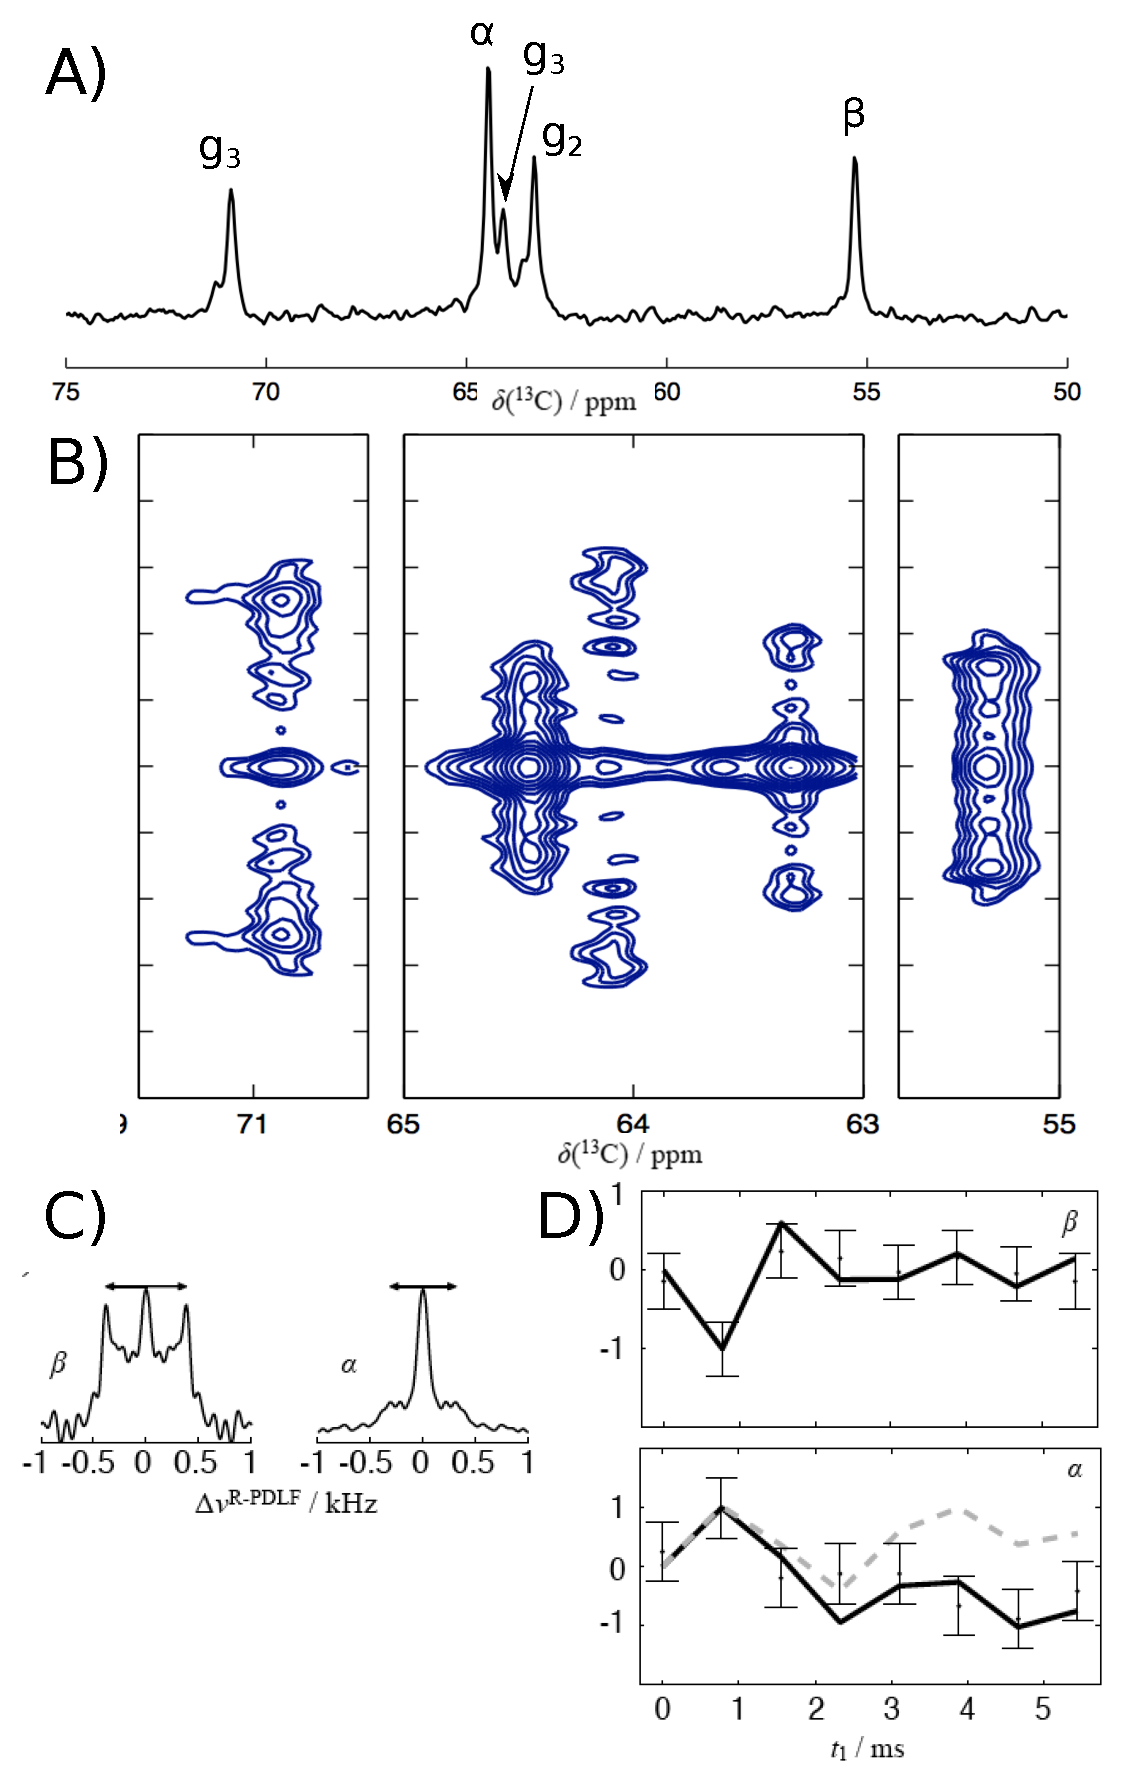
\includegraphics[width=8.5cm]{../scratch/figIDEA.eps}
  \caption{\label{PShgSIGNSsimpson}
    (a) The headgroup region of the INEPT spectrum with headgroup and glycerol backbone carbons assigned.
    (b) 2D R-PDLF spectra for headgroup and glycerol backbone regions.
    (c) Slices for $\alpha$ and $\beta$ barbons.
    (d) Experimental SDROSS data (points) and SIMPSON simulations (lines).
    Order parameter values of -0.12 for the $\beta$-carbon, and 0.09 and -0.02
    for the larger and smaller $\alpha$-carbon slittings were used in the
    SIMPSON calculations. The S-DROSS curve from SIMPSON simulation with positive value
    for the smaller order parameter (dashed grey).
  }
  \todo{This is preliminary figure, should be polished.} \\
  \todo{Should we show slices for all the analyzed carbons in (c)?}
\end{figure}

%\begin{figure}[!htb]
%  \centering
%  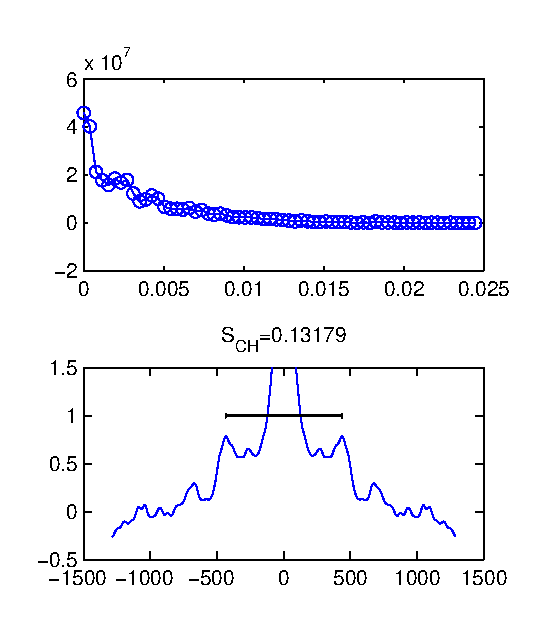
\includegraphics[width=5.5cm]{../Figs/g1_slice_large.eps}
%  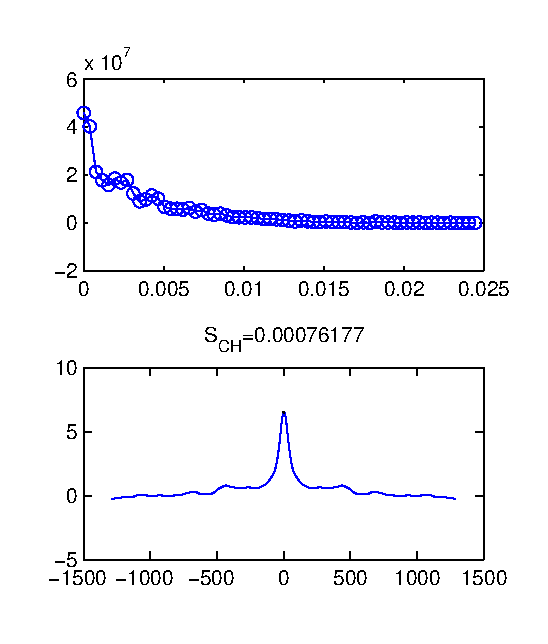
\includegraphics[width=5.5cm]{../Figs/g1_slice_small.eps}
%  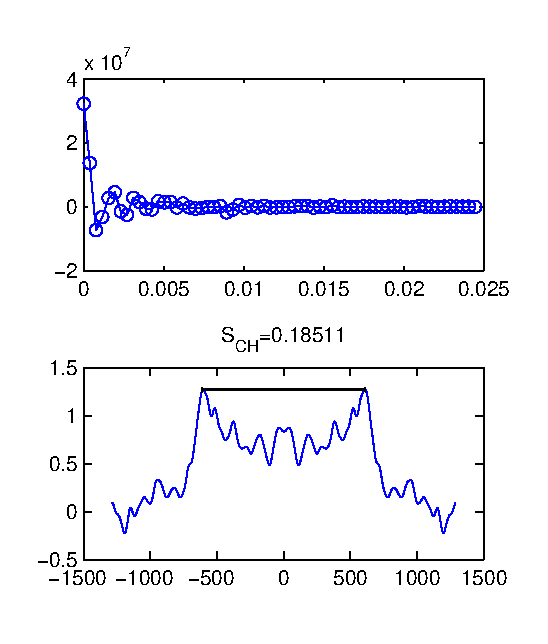
\includegraphics[width=5.5cm]{../Figs/g2_slice.eps}
%  \caption{\label{glycerolNMR}
%    R-PDFL slices for gycerol backbone carbons.
%  }
%  \todo{We need nicer figure for this data. Maybe combine with \ref{PShgSIGNSsimpson}} \\
%  \todo{What are the top figures actually?}
%\end{figure}

The headgroup and glycerol backbone order parameters of 
POPS measured in this work are in good agreement with the previously reported
values from $^2$H NMR experiments of DOPS \cite{browning80} (Fig. \ref{HGorderParameters}).
The $\beta$-carbon order parameter is significantly more negative and $\alpha$-carbon
experiences a significant forking in PS headgroup when compared with
the values previously measured for POPC \cite{ferreira13} (Fig. \ref{HGorderParameters}).  
These features have been intepreted to arise from a rigid PS headgroup
conformation, stabilized by hydrogen bonds or electrostatic
interactions \cite{browning80,buldt81}, but detailed structrural interpretation is not
available. 
%The detailed structural differences between the headgroups is, however, not known.
\begin{figure}[]
  \centering
  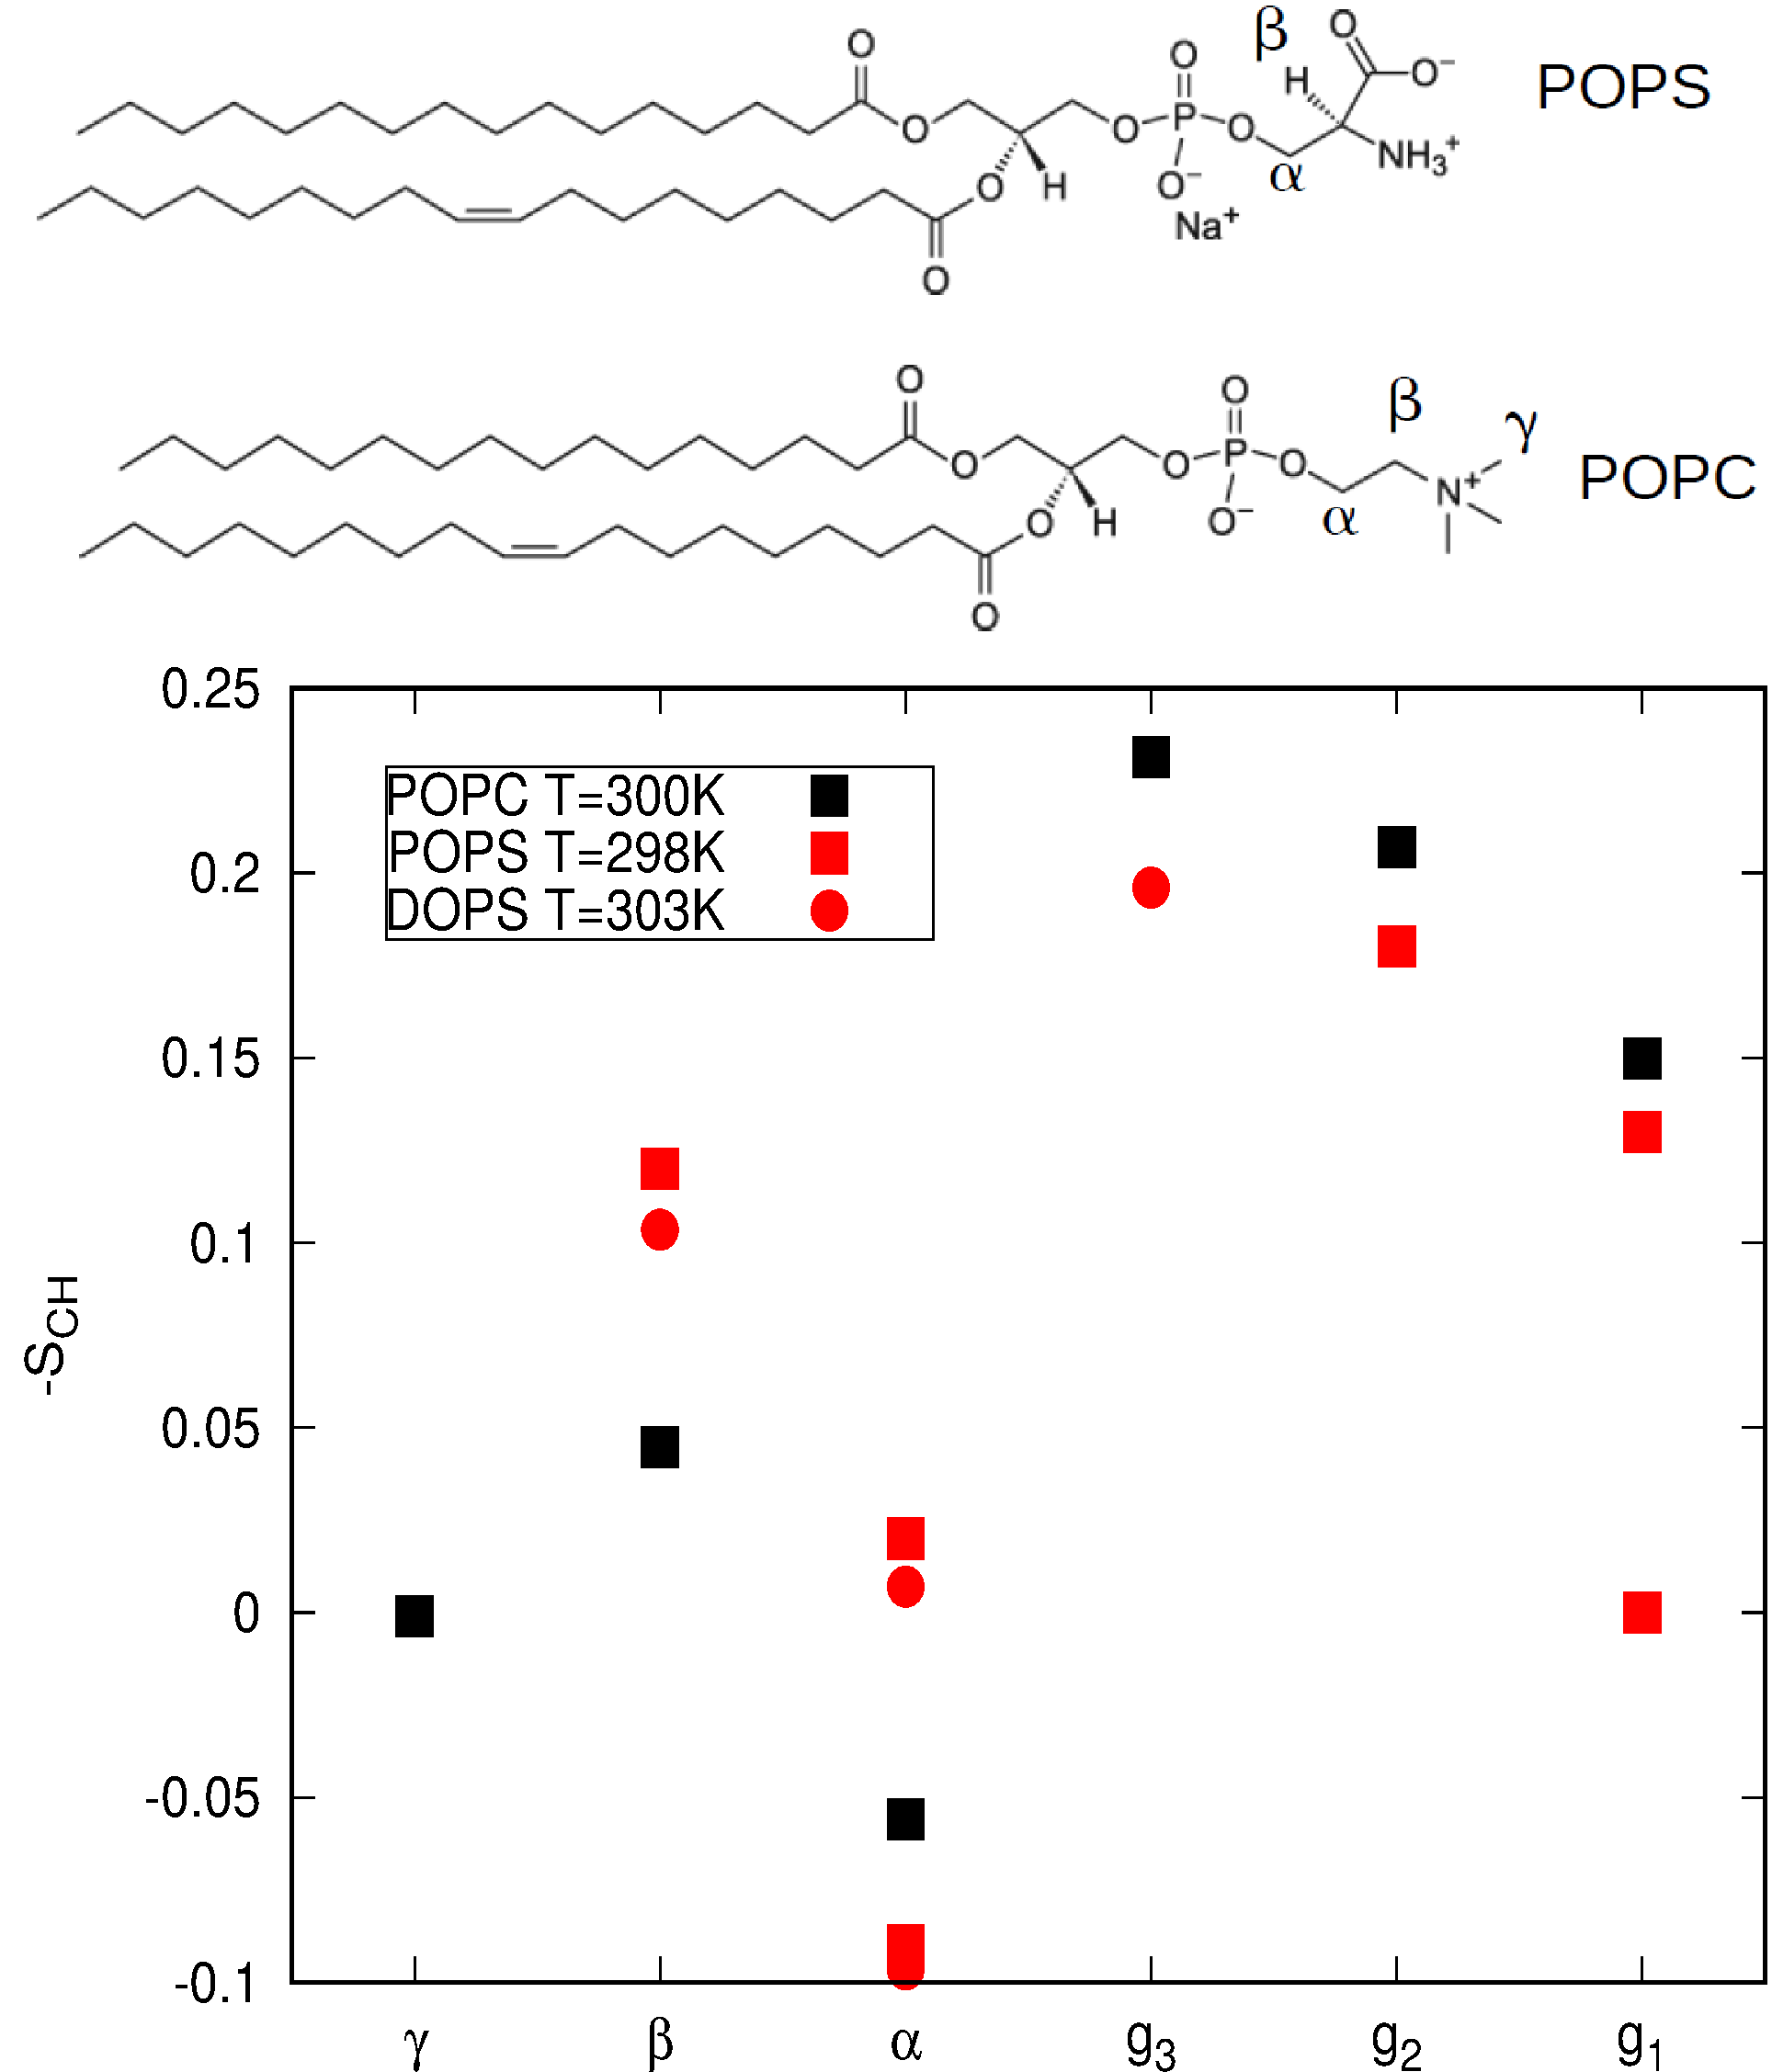
\includegraphics[width=9.0cm]{../Figs/PCPScomp.pdf}
  \caption{\label{HGorderParameters}
    Headgroup and glycerol backbone order parameters of POPS measured in this work compared
    with the values from DOPS ($^2$H NMR, 0.1M of NaCl) \cite{browning80} and 
    POPC  ($^{13}$C NMR) \cite{ferreira13} experiments. Signs of the PS order parameters
    are measured in this work. Signs of the PC order parameters are measured in Ref.~\cite{ferreira16}.
  }
\end{figure}


%\begin{figure}[]
%  \centering
%  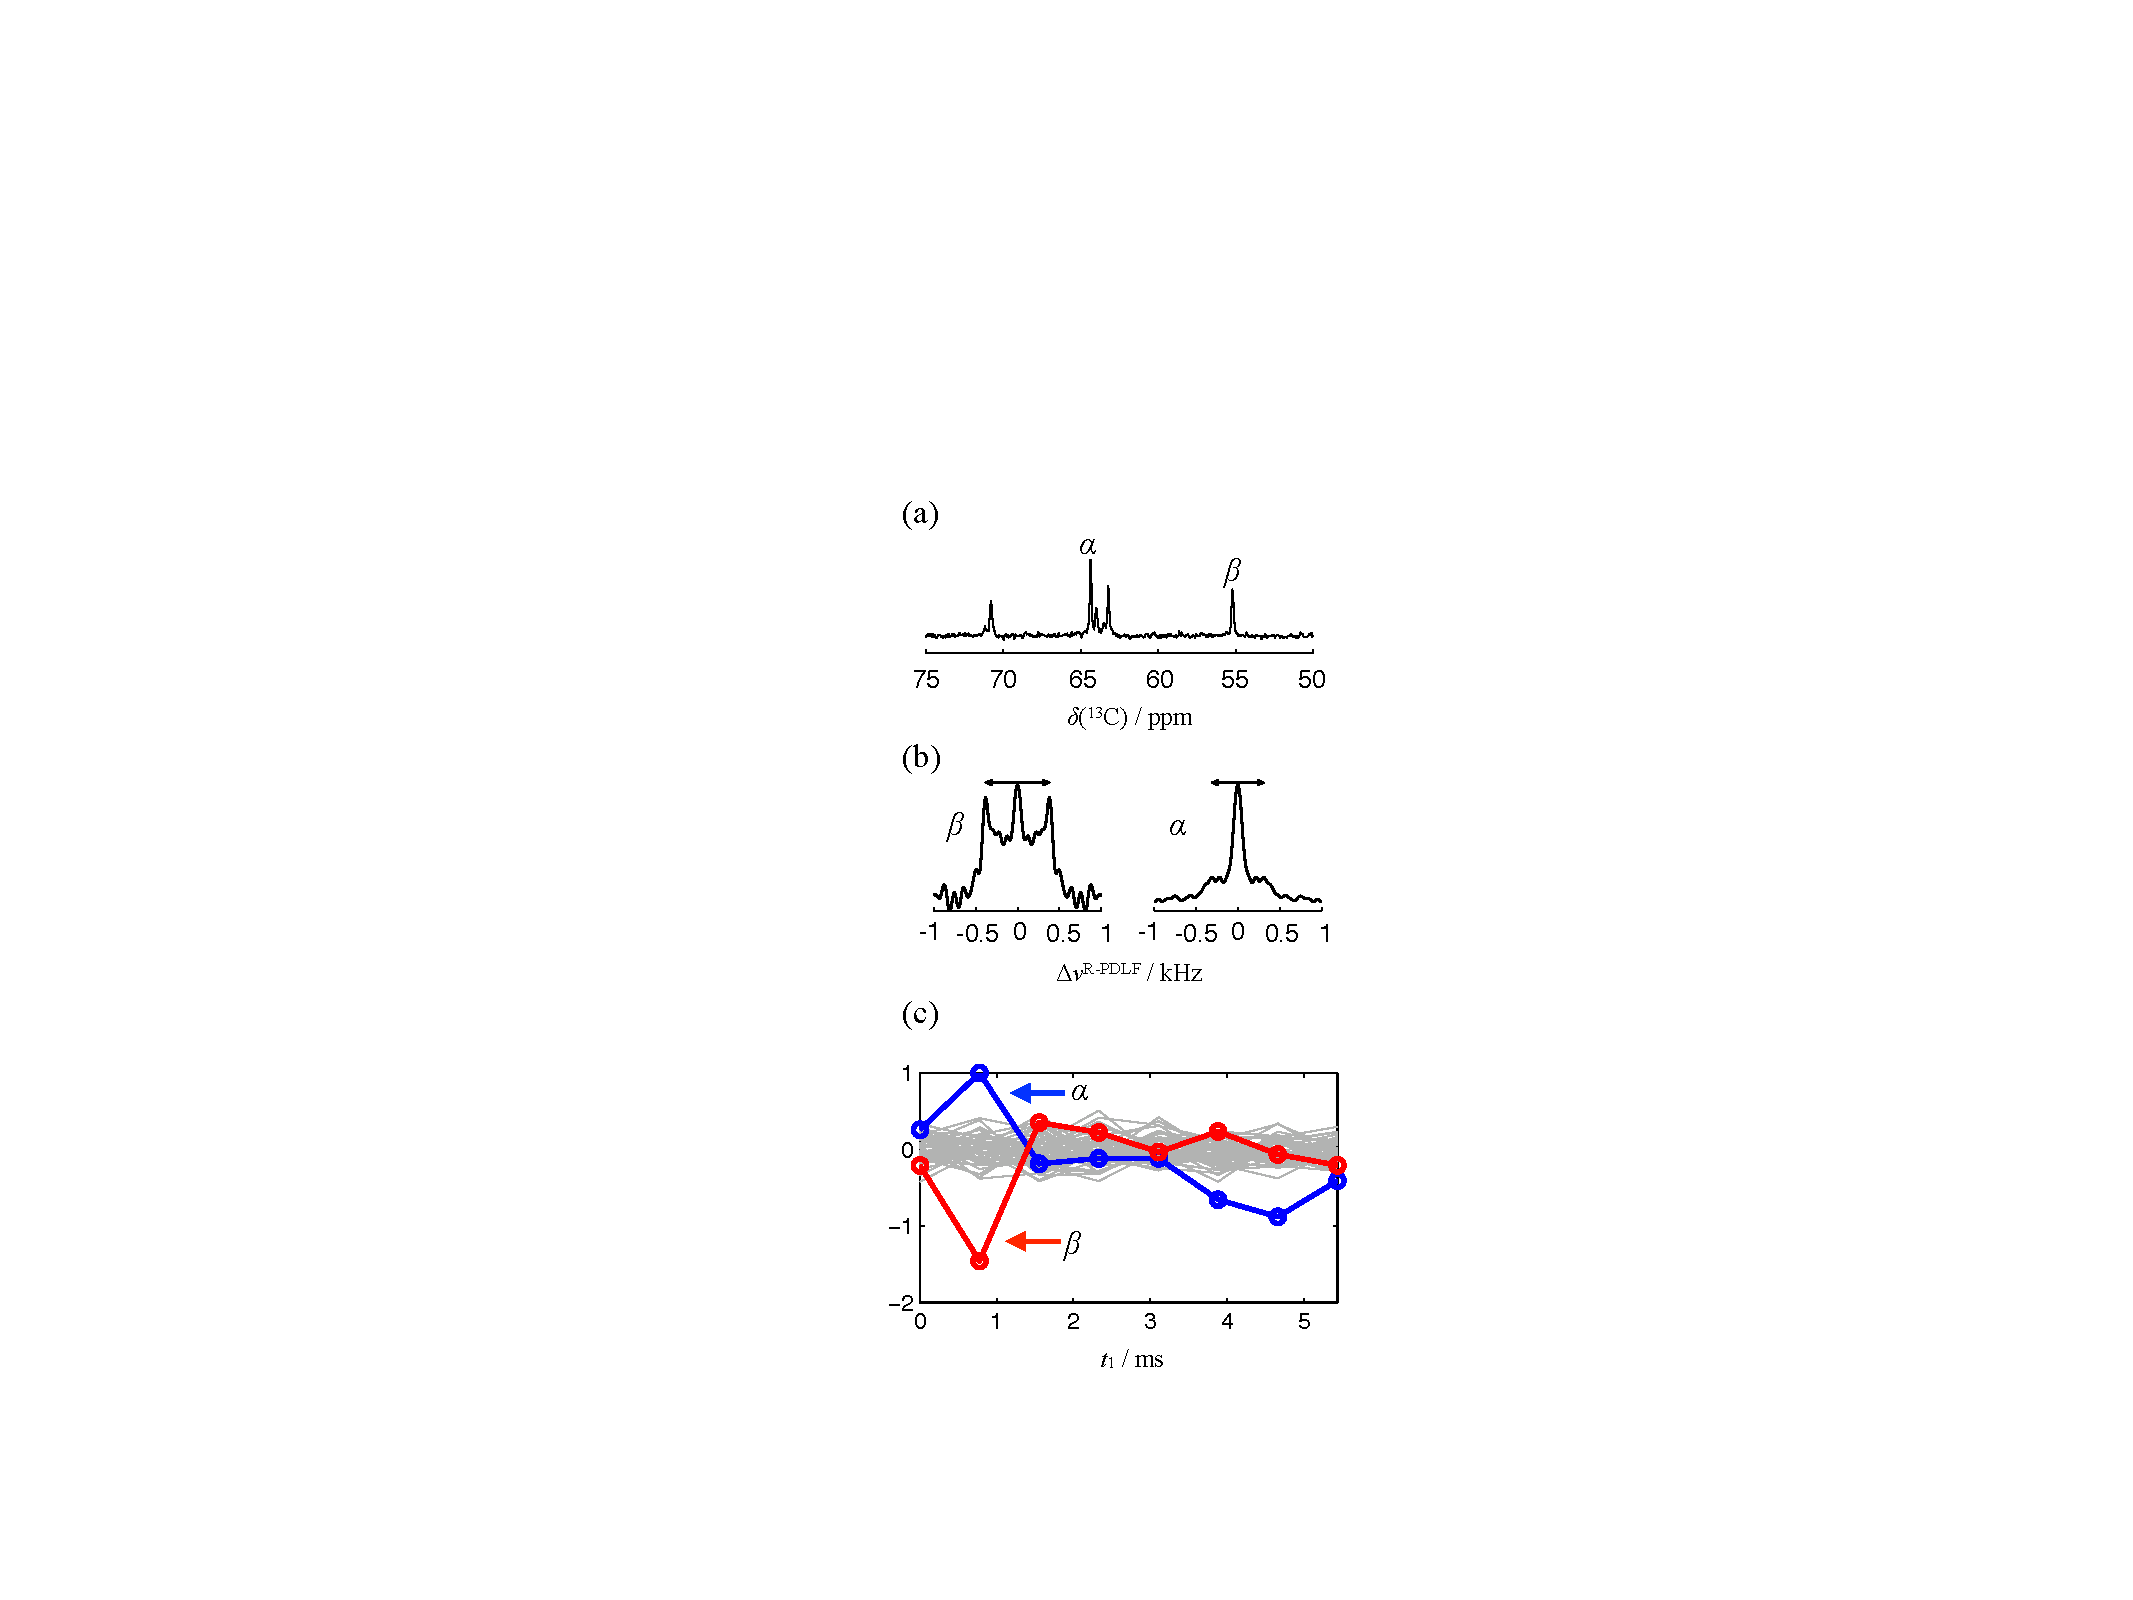
\includegraphics[width=9.0cm]{../Figs/PShgSIGNS.pdf}
%  \caption{\label{PShgSIGNS}
%    Experimental results for sign measurement for POPS sample
%  }
%\end{figure}


\subsection{Headgroup and glycerol backbone in simulations of PS lipid bilayers without additional ions}
\begin{figure}[]
  \centering
  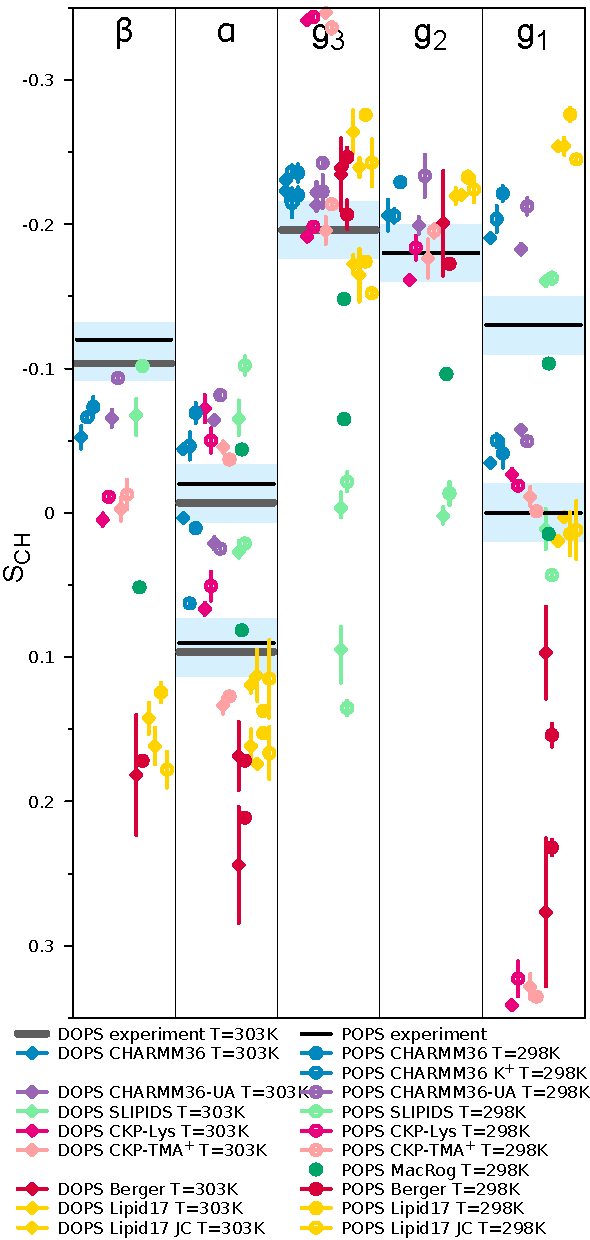
\includegraphics[width=9.0cm]{../Figs/HGorderparametersPS.pdf}
  \caption{\label{HGorderParametersPS}
    Order parameters for PS headgroup and glycerol
    backbone from simulations with different models and experiments without CaCl$_2$.
    All DOPS data at 303~K, POPS at 298~K.
    Experimental data from \cite{browning80} contain 0.1~M of NaCl.
    Signs are taken from experiments for POPS described in Supplementary Information.
    The vertical bars shown %for most computational values
    are not error bars, but demonstrate that %for these systems
    we had at least two data sets; the ends of the bars mark the extreme values from the sets, and the dot marks their measurement-time-weighted average.
  }
\end{figure}

\begin{figure}[]
  \centering
  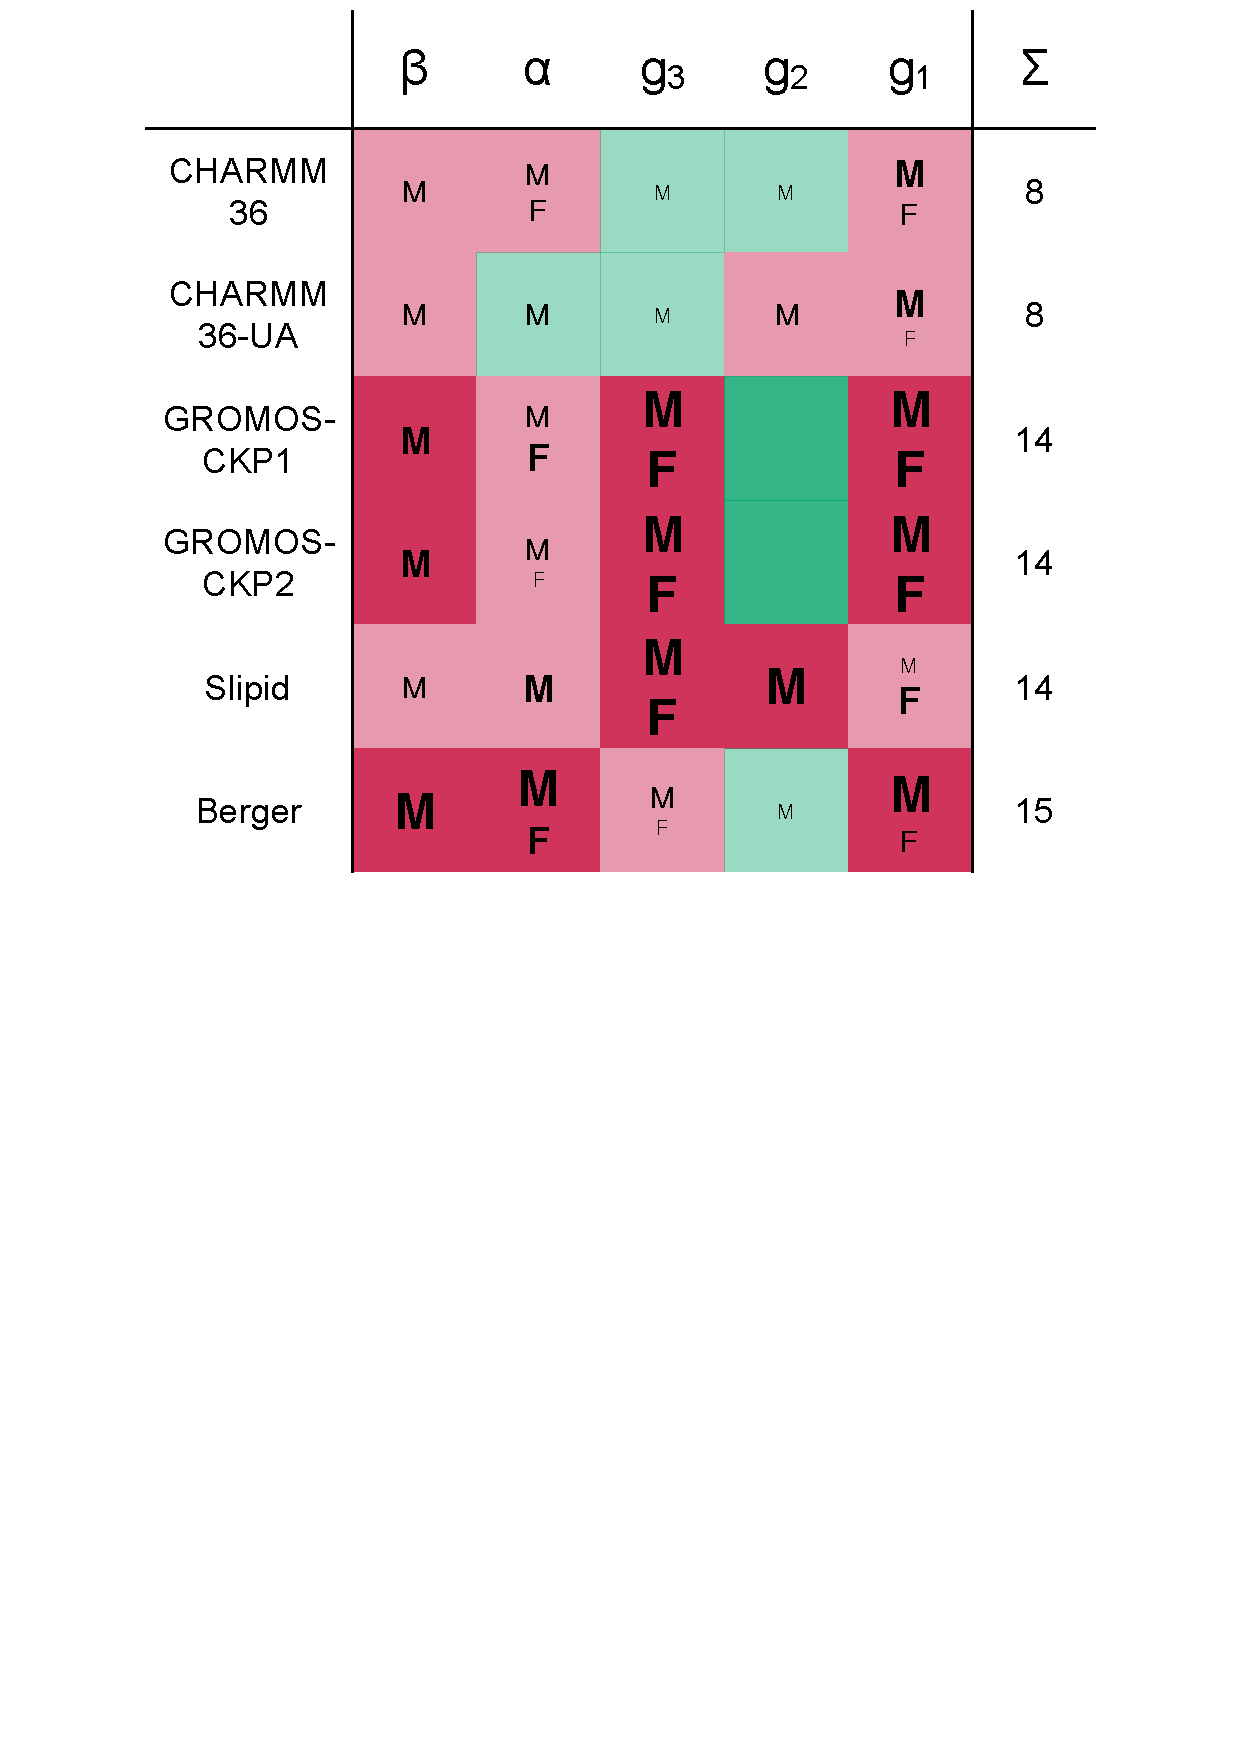
\includegraphics[width=9.0cm]{../Figs/comparisonTablePS.pdf}
  \caption{\label{comparisonTablePS}
  Rough subjective ranking of force fields based on Figure~\ref{HGorderParametersPS}. Here ÒMÓ indicates a magnitude problem, ÒFÓ a forking problem; letter size increases with problem severity. Color scheme: Òwithin experimental errorÓ (dark green), Òalmost within experimental errorÓ (light green), Òclear deviation from experimentsÓ (light red), and Òmajor deviation from experimentsÓ (dark red). The $\Sigma$-column shows the total deviation of the force field, when individual carbons are given weights of 0 (matches experiment), 1, 2, and 4 (major deviation). For full details of the assessment, see Supplementary Information.
  }
  \todo{Issue about possible updates to this plot: https://github.com/NMRLipids/NMRlipidsIVotherHGs/issues/4} \\
  \todo{Lipid17 and MacRog results should be added into this plot.}
\end{figure}

None of the tested models reproduce the experimental headgroup and 
glycerol backbone order parameters of DOPS and POPS within the
experimental error bars (Fig. \ref{HGorderParametersPS}). 
The tested models perform generally less well than the models tested
for PC headgroup in the previous study (Fig. 2 in Ref.~\cite{botan15}),
which is also evindent from the comparison between subjective rankings
of the model quality for the headgroup and glycerol backbone 
(Fig. \ref{comparisonTablePS} and Fig. 4 in Ref.~\cite{botan15}).
Therefore, the models cannot be straightforwardly used to interpret the
structural differences between PC and PS headgroups. 
However, the differences are partially reproduced by the two best performing 
models for the $\alpha$ and $\beta$-carbons of PS headgroups, Slipids and CHARMM36.
Both reproduce the larger forking of the $\alpha$-carbon 
and the Slipids model reproduces also the lower of the $\beta$-carbon order 
in parameter in the PS headgroups (Fig. \ref{HGorderParametersPS} and Fig. 2 in Ref.~\citenum{botan15}).
Interestingly, the dihedral angle distributions 
%of CHARMM36 and Slipids in 
in these two models share significant similarities in the headgroup region (Fig.~\ref{dihedralsHG}). 
\todo{Notation of dihedrals in Fig.~\ref{dihedralsHG} should be made somehow combatible with the
chemical structures in Fig.~\ref{HGorderParameters} and the discussion should be then finished.}
However, the glycerol backbone order parameters in Slipids model
significantly differ from CHARMM36 results and experiments (Fig. \ref{HGorderParametersPS}),
which can be related to the differences in the dihedral angle distributions 
of C1-C2-C3-O31 and C2-C3-O31-C31 (Fig.~\ref{dihedralsGLY}). 
Similar difference was previously observed for PC lipids \cite{botan15}
and the conformational differences are illustrated in Figure \ref{glycerol_buslaev}. 

%\todo{Discussion is to be finished.
%  One possible conclusion could be the following:
%  The main differences between the models in the headgroup region are observed
%  for dihedrals C12-C11-O12-P and C11-C12-C13-O1A.
%  CHARMM36, CHARMM36UA and Slipids give very similar results to the
%  dihedral C11-C12-C13-O1A, which is close to the $\beta$-carbon.
%  The order parameters of $\beta$-carbons for these three models
%  are in best argeement with the experiments in figure \ref{HGorderParametersPS}.
%  On the other hand, Gromos-CKP models give better order parameters
%  for $\alpha$-carbon than Slipids, CHARMM36 or CHARMM36UA. 
%  In conclusion, the suggestion would be that the single peak for
%  observed at 120 degrees in CHARMMs and Slipids would
%  be more realistic for C11-C12-C13-O1A dihedral, while the single peak at 180 degrees observed
%  in CKP models and in Berger would be most realistic for C12-C11-O12-P dihedral.
%}

\todo{POPS/OPPS issue with MacRog model is in progress: https://github.com/NMRLipids/NMRlipidsIVotherHGs/issues/16}

%
%The total deviation from the experiments ($\Sigma$ in Fig. \ref{comparisonTablePS})
%for the best performing CHARMM36 model is larger for PS lipids (8)
%than for PC (3) \cite{botan15}.
%Therefore the interpretation of structural details of PS headgroup or
%differences between PC and PS lipids is very challenging 
%from the current MD simulation models.


\subsection{Counterion binding to lipid bilayers containing PS lipids}
Membranes containing PS lipids are always accomppanied with counterions, which
modulate electrostatic interactions between lipids and other biomolecules. 
Counterions are also suggested screen the repulsion between charged lipid headgroups 
in MD simulations and reduce the area per lipid of PS bilayers to be smaller than in PC
bilayers~\cite{pandit02,mukhopadhyay04,pedersen06}. 
The counterion density profiles along membrane normal 
show significant differences between simulation models (Fig. \ref{NAdensPOPS}).
The strongest counterion binding, i.e., the lowest concentrations in bulk water,
are observed in MacRog, Berger and Lipid17/JC simulations.
CHARMM36, CHARMM36ua and Gromos-CKP models exhibit two local maxima in counterion
density, while a single maxima is observed in the other models. 
\todo{More detailed discussion may be possible after comparing monovalent ion binding
to bilayers between CHARMM simulations and experiments.
Also, section S6 should be finished.}
Area per lipid is in agreement with experiments \cite{pan14} only
in the Gromos-CKP models, while other models give significantly lower values (Fig. \ref{NAdensPOPS}).
The difference cannot be explained by the electrostatic screening of the headgroup repulsion due to 
counterion binding because CHARMM36, CHARMM36ua and Slipid models give
smaller area per lipid than Gromos-CKP models with similar counterion binding affinity.
%The proposed trend is observed for Lipid17 model,
%for which the Joung-Cheatham ions give higher affinity and smaller area
%per molecule. However, the trend is not observed when comparing accross different
%force fields. For example, CHARMM36ua and MacRog give similar area per molecule
%but binding affinity is significantly higher in MacRog. 
\begin{figure}[]
  \centering
  \includegraphics[width=9.0cm]{../Figs/NAdensPOPS.eps}
  \caption{\label{NAdensPOPS}
    Counterion densities of POPS lipid bilayer along the membrane normal from
    simulations with different force fields.
  }
\end{figure}

To evaluate counterion binding in different simulation models against experimental data~\cite{roux90},
we plot the headgroup order parameters measured from POPC:POPS 5:1 mixture
as a function of different monovalent ions added to the buffer (Fig. \ref{PSresponseTONaCl}). 
Experimental order parameter data for POPC headgroup in the mixture is available as a function
of LiCl and KCl concentrations, while POPS headgroup order parameters are measured also
as a function of NaCl. Lithium interacts more strongly with PS headgroups than other monovalent 
ions~\cite{hauser83,hauser85,roux86,mattai89,roux90}, as also observed for PC headgroups~\cite{cevc90}. 
This is evident also in the changes of PS headgroup order parameters, which decrease with the addition of lithium 
but increase with the addition of sodium or potassium (Fig. \ref{PSresponseTONaCl}). 
POPC headgroup order parameters exhibit a clear decrease as a function of LiCl concentration
but only modest changes as a function of KCl concentration, indicating singificant 
Li$^+$ binding but only weak Na$^+$ binding to the mixture when interpreted using the
electrometer concept~\cite{akutsu81,altenbach84,seelig87}. In simulations with the
Berger model, the headgroup order parameter response of POPC
to the added NaCl is similar to the experiments of LiCl,
indicating overestimated binding affinity of sodium, in line with the results for PC bilayers \cite{catte16}.
Indeed, the sodium density profile shows a significant binding peak in the 
Berger model (Fig. \ref{CIdensPSOCmixt}). Potassium binding in the MacRog simulation
is significantly weaker  (Fig. \ref{CIdensPSOCmixt}) and the headgroup order parameter 
changes are also in better agreement with simulations (Fig. \ref{PSresponseTONaCl}).
\todo{Discussion about Lipid17 to be written when we have the density profiles.}
All the tested models overestimate the changes of POPS headgroup order parameters as
a function of monovalent ions (Fig. \ref{PSresponseTONaCl}), suggesting that
model development is necessary to interpret the PS headgroup-ion interactions 
from MD simulations.
\begin{figure*}[]
  \centering
  \includegraphics[width=18.0cm]{../Figs/CHANGESwithMONVALENTwithPS.eps}
  \caption{\label{PSresponseTONaCl}
    Changes of the PC (left) and PS (right) headgroup order parameters as a function of
    added NaCl, KCl and LiCl from POPC:POPS (5:1) mixture. The experimental data is from Ref. \citenum{roux90}.
    The values from counterion-only systems are set as a zero point of y-axis.
    To correctly illustrate the significant forking of the $\alpha$-carbon order parameter
    in PS headgroup (bottom, right), the y-axis is tranferred with the same value for both order parameters such that the lower order
    parameter value is at zero.
  }
  \todo{CHARMM36 results for this plot would be highly useful.}
\end{figure*}


\begin{figure}[]
  \centering
  \includegraphics[width=8.0cm]{../Figs/CIdensPSOCmixt.eps}
  \caption{  Counterion density distributions from PC:PS mixtures.
\label{CIdensPSOCmixt}
  }
  \todo{Lipid 17 is to be added.}
\end{figure}




\subsection{Headgroup structure in PS and PC mixtures}
Dilution of PS lipid bilayers with PC lipids reduces the propensity
of PS headgroup-multivalent ion complexes and is proposed to make PS
headgroups less rigid~\cite{browning80,buldt81,roux90,roux91}.
Therefore, the intermolecular interactions at the headgroup region seems
to be important for the physical properties of mixed lipid bilayers.
These interactions can be indirectly monitored by measuring the
headgroup order parameters from PS:PC mixtures with different molar
ratios. The headgroup order parameters of POPC increase in such experiments 
with increasing amount of POPS (Fig.~\ref{HGorderparametersPCvsPS})~\cite{scherer87}. 
This behaviour is generally observed when negatively charged lipids or surfactants 
are mixed with PC lipids~\cite{scherer87,scherer89} and can be understood by the 
tilting of lipid headgroup more parallel to the membrane plane according to
the electrometer concept \cite{seelig87}. The headgroup order parameters of PS lipids
shift closer to zero when bilayer is diluted with PC lipids in 
experiments (Fig.~\ref{HGorderparametersPCvsPS})~\cite{browning80,scherer87,roux90},
which is intepreted to indicate reduced rigidity~\cite{browning80,buldt81}.

The increase of POPC headgroup order parameters with the increasing
amount of negatively charged POPS lipid is reproduced in
MacRog simulations with potassium counterions, but not in 
Berger simulations with sodium or in CHARMM36 simulations
with potassium or sodium conterions (Fig. \ref{HGorderparametersPCvsPS}). 
The observations can be explained using the electrometer concept.
The Berger simulation exhibits very strong sodium binding (Fig. \ref{CIdensPSOCmixt}), 
which surpasses the effect of negatively charged lipids as also the amount of
counterions increase with increasing amount of PS.
In CHARMM36 simulations, the counterion binding neutralizes the effect
of PS and the headgroup order parameters are not changed with increasing amount
of PS. Finally, the weak binding of potassium in the MacRog simulations
enables the increase of order parameters with the increasing amount of
negatively charged PS lipids (Figs. \ref{HGorderparametersPCvsPS} and \ref{CIdensPSOCmixt}).

\begin{figure*}[]
  \centering
  \includegraphics[width=16.0cm]{../Figs/HGorderparametersPCvsPS.eps}
  \caption{\label{HGorderparametersPCvsPS}
    Changes of PC (left panel) and PS (right panel) headgroup order parameters
    from POPC:POPS mixtures with increasing amount of POPS.
    Experimental results of POPC are taken from Ref. \citenum{scherer87}
    (signs are determined as discussed in \cite{botan15,ollila16}).
    Experimental values for POPS in pure bilayer and in mixture are  
    measured in this work and in Ref. \citenum{roux90} at 298K, respectively.
    Since the experimental data of POPS in pure and diluted mixture come from
    different experimental sets (13C NMR in this work and 2H NMR from Ref. \citenum{roux90}),
    the experimental change of the order parameter is less accurate than in typical measurements
    where same technique is used in all conditions, see discussion about qualitative and quantitative 
    accuracy in Ref. \citenum{ollila16}.
    For POPC (left panel) the zero point of y-axis is set to the value of pure bilayer.
    For $\beta$-carbon of POPS (right panel, top) the zero point of y-axis is
    set to the value from POPC:POPS (5:1) mixture.
    For $\alpha$-carbon of POPS (right panel, bottom) the y-axis is tranferred
    with the same value for both order parameters such that the lower order
    parameter value from POPC:POPS (5:1) mixture is at zero
    to correctly illustrate the significant forking.
  }
  \todo{Simulation of CHARMM36 at 298K should be maybe rerun with Gromacs 5.} \\
  \todo{Simulation of pure POPC at 298K with Lipid14 would be useful for this plot (only at 303 K is available from NMRlipids I)} \\
  \todo{MacRog simulations of pure POPS with potassium counterions only would be useful for this and other plots.} \\
  \todo{The data from POPC used in Gromos-CKP by would be useful for this plot.}
\end{figure*}

Oppositely to experiments, the headgroup order parameter of POPS shift away
from zero in CHARM36 simulations when bilayer is diluted with POPC (Fig. \ref{HGorderparametersPCvsPS}).
In lipid14/17 simulations, the POPS order parameter shift closer to zero when
bilayer is diluted with POPC, but the numerical values of order parameters
are too far from experiments to enable interpretation of the experimental data.
Therefore, we conlcude that the force field development is necessary before
MD simulations can be used to interpret the interactions between PC and PS headgroups.
%The $\beta$-carbon order parameter
%increase with increasing amount of PS in CHARMM36 and MacRog simulations in contrast
%to the experimental data.
%The smaller $\alpha$-carbon order parameter increase in both
%simulation models with increasing amount of PS, while it is almost unchanged in experiments.
%The larger $\alpha$-carbon order parameter increase in MacRog and decrease in CHARMM36
%with increasing amount of PS, both model exhibiting a poor agreement with experiments. 



\subsection{Ca$^{2+}$ binding affinity in bilayers with negatively charged PS lipids}

Ion binding affinity to PS containing membranes can be most conveniently measured 
from PC:PS lipid mixtures where the lipid-ion complexes and phase separation are 
not observed \cite{feigenson86,mattai89,roux90,roux91}. Also, the headgroup order 
parameters of PC can be used to detect ion binding affinity to the mixed lipid 
bilayers, see section~\ref{electrometerFORmixtures}. As expected from the previous study of PC lipid bilayers \cite{catte16}, 
the decrease of POPC headgroup order parameters in POPC:POPS mixtures as a function of Ca$^{2+}$ concentration 
is overestimated with respect to experiments \cite{roux90} in almost all the 
tested simulation models (Fig. \ref{changesWITHCaClPS}), indicating overestimated calcium binding
binding affinity. Only exception is the CHARMM36 model with the special NBfix~\cite{kim16} interaction, 
incorporated in the parameters give by the CHARMM-GUI at the time of running the simulations (January 2018),
which underestimates the calcium binding affinity. With this interaction, the 
calcium and sodium binding affinities to POPC bilayer are equally weak (see section S7), in contrast to experimental 
data~\cite{cevc90,akutsu81,altenbach84}. Therefore, we conclude that the ion binding peaks in
density distributions along membrane normal (Fig. \ref{CAdensPCPSmixture}) are underestimated 
in the CHARMM36/NBfix model, but overestimated in the other tested models.

%It should be noted, however, that the lowest concentration (100mM) gives
%a good agreemet with experiments
%\todo{Should be analyze/discuss this further?
%  Binding with $\sim$100 mM is saturated in both Berger and MacRog simulations. Maybe this is realistic?
%It should be noted that Berger simulation do not have counterions.}.

\begin{figure*}[]
  \centering
  \includegraphics[width=18cm]{../Figs/CHANGESwithCaClPS.eps}
  \caption{\label{changesWITHCaClPS}
    Changes of POPC (left) and POPS (right) headgroup order parameters in POPC:POPS (5:1) mixture
    as a function CaCl$_2$ concentration. Experimental data is taken from \citenum{roux90}.
    The values from counterion-only systems are set as a zero point of y-axis.
    To correctly illustrate the significant forking of the $\alpha$-carbon order parameter
    in PS headgroup (bottom, right), the y-axis is tranferred with the same value for both order parameters such that the lower order
    parameter value is at zero. 
  }
  \todo{Information about the cuonterions in different simulations should be added} \\
  \todo{Upcoming simulations with original CHARMM36 have been mentioned in the blog:
  http://nmrlipids.blogspot.com/2017/12/nmrlipids-iv-current-status-and.html?showComment=1520090718976\#c5569269391707740056} \\
  \todo{Upcoming Lipid17 simulations have been mentioned in the blog
    http://nmrlipids.blogspot.com/2017/12/nmrlipids-iv-current-status-and.html?showComment=1515177306419\#c994825612316235467}
\end{figure*}

\begin{figure}[]
  \centering
  \includegraphics[width=9cm]{../Figs/CAdensPCPSmixture.eps}
  \caption{\label{CAdensPCPSmixture}
    Ca2+ density profiles from simulations.
  }
  \todo{The CHARMM results are mass densities, numbers should be used.} \\
  \todo{Should we include also counterions into the plot?} \\
  \todo{Not all the data from MacRog is included.} 
\end{figure}

The headgroup order parameters of POPS headgroup measured from POPC:POPS (5:1) mixture
exhibit a strong dependence of CaCl$_2$ with small concentrations with a rapid saturation
below 100 mM (Fig. \ref{changesWITHCaClPS}). The $\beta$-carbon order parameter of
POPS increase with the added CaCl$_2$ in the experiment and in all the tested simulation models,
but simulations significantly overestimated the change. The larger $\alpha$-carbon order
parameter of POPS decrease and the smaller one slightly increase with the added
CaCl$_2$ in the experiment. The changes are again significantly overestimated in
the simulations, however, in this case all simulations predict qualitatively different
behaviour. Notably, the changes of POPS headgroup order parameters are overestimated
also in the CHARMM36/NBfix model where the calcium binding affinity was too low. 
We conclude that the effect of bound ions to the headgroup order parameters of POPS
is not qualitatively reproduced by the tested simulations models. This is in contrast
to previous results for PC headgroup \cite{catte16}, where qualitatively correct reponse to bound ions was
observed despite of significant discrepancies in the headgroup structure without additional ions. 
The response of POPS headgroup order parameters to the bound charge is systematic but
less well understood than the responce of PC headgroups used in the electrometer
concept \cite{seelig87,roux90}. The force field development is necessary to
generate MD simulations that could be used to explain the interactions between
PS headgroup and calcium ions.


\section{Conclusions}
We have collected a set of experimental NMR order parameter data,
which could be combined with MD simulations to interpret the
headgroup structure and cation binding details to negatively charged
membranes containing PS lipids. Using open collaboration method, we
tried to find a MD simulation model which would be sufficiently accurate
to interpret the experimental data. However, none of the tested models
was accurate enough. In line with the previous study for PC lipids \cite{catte16},
MD simulation models seems to generally overestimate cation binding also
to negatively charged bilayers containing PS lipids, with some exceptions.
The response of PS lipid headgroup order parameters to the bound cations
does not agree with experiments, even in the cases where binding affinity is
not overestimated. This is in contrast to the previous results with PC lipids,
where the qualitative response of the headgroup order parameters was in agreement
with experiments even in the cases where the headgroup structure without ions was not
correct and the cation binding affinity was overestimated. In addition, the inaccurate
responses of PS headgroup order parameters to the dilution with PC lipids suggests
that the PC-PS interactions are not accurately described by the tested models.

Our results pave the way for improving the PS lipid parameters for MD simulations
by offering the set of experimental data for the quality measurement, by
pinpointing problems areas in the models and suggesting directions for the corrections.
Improvements using the electronic continuum correction is already in progress \url{https://github.com/jmelcr/ecc_lipids},
following the recent work for PC lipids \cite{melcr18}.

% Tables may be be put in the text as floats.
% Here is an example of the general form of a table:
% Fill in the caption in the braces of the \caption{} command. Put the label
% that you will use with \ref{} command in the braces of the \label{} command.
% Insert the column specifiers (l, r, c, d, etc.) in the empty braces of the
% \begin{tabular}{} command.
%
% \begin{table}
% \caption{\label{} }
% \begin{tabular}{}
% \end{tabular}
% \end{table}

% If you have acknowledgments, this puts in the proper section head.
\begin{acknowledgments}
% Put your acknowledgments here.
\end{acknowledgments}

\newpage


% Create the reference section using BibTe
\bibliography{refs.bib}

%\newpage
%\section{APPENDIX: The NMR results reported by Tiago Ferreira}

\listoftodos

\end{document}
%
% ****** End of file aiptemplate.tex ******
